% ============================================================
% ScribbleDB: Natural Language to Relational Database Synthesis
% Skeleton draft -- headings, placeholders, algorithm stubs
% ============================================================
\documentclass[sigconf]{acmart}

\usepackage{algorithm}
\usepackage{algpseudocode}
\usepackage{booktabs}
\usepackage{multirow}
\usepackage{enumitem}
\usepackage{listings}

\lstset{
  language=Python,
  basicstyle=\small\ttfamily,
  breaklines=true,
  frame=single,
  xleftmargin=4pt,
  xrightmargin=4pt
}

% Shorthand for comparison table
\newcommand{\yes}{$\checkmark$}
\newcommand{\no}{$\times$}
\newcommand{\partsup}{$\circ$}   % partial support

\begin{document}

% ---- Draft / copyright suppression ----
\setcopyright{none}
\acmConference[SIGMOD '27]{ACM SIGMOD International Conference on Management of Data}{2027}{TBD}
\acmDOI{10.1145/XXXXXXX.XXXXXXX}
\acmISBN{XXX-X-XXXX-XXXX-X/27/00}

% ---- Title ----
\title{ScribbleDB: Natural Language to Relational Database Synthesis}

% ---- Authors ----
\author{Aviroop Mitra}
\email{aviroopmitra@iisc.ac.in}
\affiliation{%
  \institution{Indian Institute of Science}
  \city{Bengaluru}
  \country{India}
}

\author{Anupam Sanghi}
\email{sanghi@iith.ac.in}
\affiliation{%
  \institution{Indian Institute of Technology Hyderabad}
  \city{Sangareddy}
  \country{India}
}

% ---- Abstract ----
\begin{abstract}
\textit{[Placeholder $\sim$150\,words. Motivate the greenfield database-generation problem: no
real data, no formal spec, only a natural-language description.
Introduce ScribbleDB as a four-stage agentic pipeline
(fact extraction $\to$ schema generation $\to$ constraint modeling $\to$ code generation)
whose output is a relational schema (DDL) plus an executable Python program that materializes
the populated tables.
Highlight the key new contributions versus prior workshop version:
(i)~deterministic inverse-function code generation for single-dependency DAG nodes,
(ii)~multivariate distribution support,
(iii)~ancestral sampling for logical constraints (FA = 1.0),
(iv)~context enrichment and shard-and-merge for scalability.
Close with headline numbers: $\sim$6$\times$ table accuracy and $\sim$4$\times$ lower latency
over SchemaAgent across three benchmark suites.]}
\end{abstract}

% ---- CCS / Keywords ----
%\ccsdesc[500]{Information systems~Database design and models}
%\ccsdesc[300]{Information systems~Database utilities and tools}
%\keywords{Database Generation; Schema Generation; Large Language Models; Agentic Pipelines; Ancestral Sampling; Constraint-based Synthesis}

\maketitle

\section{Introduction}
% ============================================================

\textit{[Para 1 --- Why synthetic databases matter: application development, testing,
benchmarking; data-privacy and greenfield constraints prevent access to real data.
Emphasise the greenfield setting: no existing deployment, no schema, no seed data.]}

\textit{[Para 2 --- State of the art and its limitations:
ab-initio generators (MUDD, PDGF, Myriad) require formal declarative specs;
regeneration-based tools (DBSynth, RSGen, Hydra, SAM) require production artefacts.
Neither suits a non-technical domain expert with only an NL description.]}

\textit{[Para 3 --- LLMs as enabler and source of new challenges.
Strong NL-to-SQL~\cite{yu2019spider} and text-to-schema~\cite{wang2025text2schema} capability.
Three core challenges for full DB synthesis:
\textbf{(a)~Expressiveness} (complex cross-table constraints),
\textbf{(b)~Hallucination} (error propagation across pipeline stages),
\textbf{(c)~Scalability} (context window degradation; materialization throughput).]}

\textit{[Para 4 --- ScribbleDB overview: how it addresses each challenge.
Emphasise that the \emph{output} is a DDL schema and an executable Python program, not
tables directly---separating correctness verification from data materialization.]}

% mention the previous paper then mention the new things
\medskip\noindent\textbf{Contributions.}
\begin{itemize}[leftmargin=*]
  \item End-to-end NL-to-database agentic pipeline; outputs relational DDL schema
        + executable Python code for table materialization.
  \item \textit{[New]} Deterministic code generation for single-dependency columns
        in the DAG via inverse functions on join/aggregate tables,
        reducing LLM calls and guaranteeing correctness-by-construction.
  \item \textit{[New, partial]} Multivariate distribution support for cross-column
        correlations beyond univariate priors.
  \item Shard-and-merge schema generation with Gale--Shapley entity alignment.
  \item Ancestral sampling for logical constraint satisfaction; FA = 1.0 empirically.
  \item Comprehensive evaluation: $\sim$6$\times$ table accuracy, $\sim$4$\times$ lower
        latency vs.\ SchemaAgent~\cite{wang2025text2schema} across three benchmark suites.
\end{itemize}

% Figure 1: Motivating example (full-width)
\begin{figure*}[t]
  \centering
  \vspace{2cm}
  \textit{[Figure 1 placeholder (full-width): Three panels.
  \textbf{Left}: NL description of the Credit Risk (Loan Origination) database.
  \textbf{Middle}: generated DDL schema excerpt (Applicants, Loans tables with PKs, FKs).
  \textbf{Right}: excerpt of rows from the materialized Loans table with the tiered
  interest-rate constraint annotated.
  Illustrates the end-to-end transformation.]}
  \vspace{2cm}
  \caption{ScribbleDB converts an NL description (left) into a relational DDL schema (middle)
           and an executable Python program whose output satisfies the stated constraints (right).
           Running example: Credit Risk (Loan Origination) database.}
  \label{fig:motivating}
\end{figure*}
% ============================================================
\section{Problem Formulation}
% ============================================================

\noindent\textbf{Definition 1 (Database Synthesis Problem).}
\textit{[Formal definition box. Input: an NL description $\mathcal{D}$ of a target database
domain plus a target row count $n$ per fact table.
Output: (i) a relational schema $\mathcal{S}$ (table definitions, primary keys, foreign keys,
data types), and (ii) a Python program $\mathcal{P}$ such that executing $\mathcal{P}$
produces a set of populated CSV/SQL tables satisfying $\mathcal{S}$ and all constraints
implied by $\mathcal{D}$.
Assumption: $\mathcal{D}$ is internally consistent (no contradiction detection).]}

\medskip
\noindent\textbf{Correctness Criteria.}
\textit{[Para: (a) Schema validity: PK uniqueness, FK referential integrity, data-type
correctness.
(b) Statistical fidelity: generated column distributions match those implied by $\mathcal{D}$
(measured by KS, MRE, NLL).
(c) Logical fidelity: all decision-tree and aggregation constraints satisfied
(measured by FA).
(d) Completeness: recall of schema elements described in $\mathcal{D}$.]}

\medskip
\noindent\textbf{Running Example.}
\textit{[Para: Introduce the \emph{Credit Risk (Loan Origination)} database as the running
example throughout the paper.
Summarise the NL description: applicants with credit scores (300--850), annual income, DTI
ratio; approved loans with an interest rate derived from a tiered lookup of credit score and
loan amount (e.g., credit score $>$ 750 \& amount $<$ \$50K $\Rightarrow$ rate $= 3.5\%$);
overall interest rate follows a Gaussian distribution.
This example is used in all stage-level figures and the case study in \S\ref{sec:eval}.]}

\section{System Architecture}
% ============================================================

\textit{[Para 1: Four-stage pipeline overview: Fact Extraction $\to$ Schema Generation $\to$
Constraint Modeling $\to$ Code Generation.
Each stage uses deterministic guard rails; failures trigger a bounded repair loop
(max 5 retries per stage).
The pipeline outputs DDL + a Python program, not tables directly, separating synthesis
from materialization.]}

\textit{[Para 2: Inter-stage interfaces. $\mathcal{F}$ = enriched fact set (JSON list of
atomic statements with tags and external-kind annotations). $\mathcal{S}$ = relational schema
(JSON: tables, columns, PKs, FKs, types). $\mathcal{C}$ = structured constraints (nested
JSON: distributions, decision trees, aggregations). $\mathcal{G}$ = column-level dependency
DAG (adjacency list). $\mathcal{P}$ = Python program (plain text).]}

% Figure 2: Architecture (full-width)
\begin{figure*}[t]
  \centering
  \vspace{2.5cm}
  \textit{[Figure 2 placeholder (full-width): ScribbleDB architecture.
  Four stage boxes arranged left-to-right with labelled inter-stage arrows
  ($\mathcal{F}$, $\mathcal{S}$, $\mathcal{C}$+$\mathcal{G}$, $\mathcal{P}$).
  Inside each box: LLM agent icon(s) + deterministic validator block + repair-loop arrow.
  Final outputs annotated: DDL schema (SQL file) and Python materialization program.]}
  \vspace{2.5cm}
  \caption{ScribbleDB architecture. Four stages connected by typed inter-stage interfaces.
           Each stage is guarded by a deterministic validator and a bounded repair loop.
           Final output: relational DDL schema and executable Python program.}
  \label{fig:architecture}
\end{figure*}

\section{Fact Extraction}
\label{sec:stage1}
% ============================================================

The initial input to the synthesis pipeline is a paragraph of natural-language prose ($\mathcal{D}$). Fact Extraction transforms $\mathcal{D}$ into a set of discrete, \emph{atomic facts} ($\mathcal{F}$). By decomposing the text, removing ambiguities, and resolving information deficiencies through targeted enrichment, this stage ensures the domain is rigorously defined before any structural modelling begins. Furthermore, extracting requirements as atomic units provides strict provenance, enabling every subsequent schema decision to be traced directly back to the specific evidence that justified it.

\subsection{Atomic Extraction and Verification}
\label{subsec:extraction}

\begin{figure}[t]
  \centering
  % If the space in the filename impedes compilation, rename the PDF to a space-free name.
  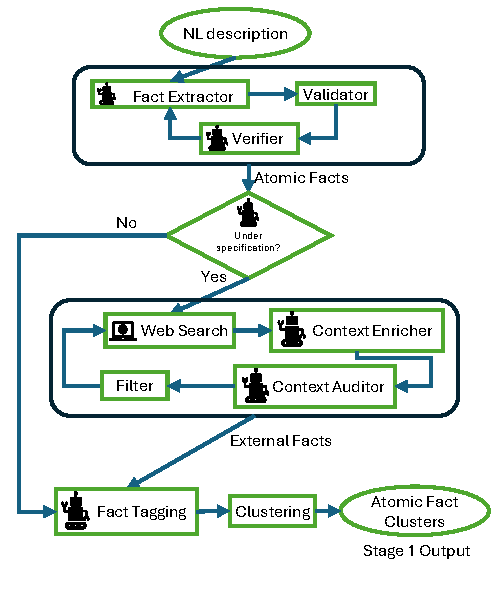
\includegraphics[width=\columnwidth,page=1]{ScribbleDB Image.pdf}
  \caption{The Fact Extraction stage. A verified set of atomic facts is gated on
  completeness; under-specified inputs are enriched against retrieved web evidence under a
  semantic auditor and a deterministic structural filter before all facts are tagged and
  clustered. The stage emits clusters of atomic facts, the sole input to Schema
  Generation (\S\ref{sec:stage2}).}
  \label{fig:stage1}
\end{figure}

An atomic fact encapsulates exactly one requirement: the existence of an entity, a specific attribute, a relationship, or a logical rule. For example, the statement ``An applicant has a credit score between 300 and 850'' is decomposed into two distinct facts: (1) an applicant has a credit score, and (2) a credit score lies between 300 and 850. This strict atomicity decouples structural definitions from logical constraints.

To ensure traceability, every fact is anchored to the specific span of $\mathcal{D}$ that justifies it. Instead of relying on an LLM to unreliably output character offsets, the extractor returns an ordered list of verbatim substrings from $\mathcal{D}$, with the atomic facts nested beneath them. Precise character offsets are then recovered via a deterministic scan.

Because initial extraction requires semantic judgement, it is delegated to an LLM agent. However, to guarantee fidelity, the output is iteratively scrutinized by a localized \emph{Dual Guard} repair loop (Figure~\ref{fig:stage1}, top). The first guard is a deterministic \textsc{Validator} that enforces structural integrity by confirming that each fact's origin segment is genuinely a verbatim substring of $\mathcal{D}$. The second guard is an LLM-based \textsc{Verifier} that identifies semantic omissions or hallucinated details. The extractor edits only the faulted facts until the audit returns clean or a retry budget is exhausted.

\subsection{Gap-Directed Context Enrichment}
\label{subsec:enrichment}

Even a fact set that is perfectly faithful to $\mathcal{D}$ may be too sparse to induce a usable schema, as initial descriptions routinely omit foundational domain knowledge. A completeness agent evaluates the verified facts against the expected structural skeleton for the target domain. If it detects severe omissions (e.g., missing core entities), it emits typed \emph{coverage gaps} and routes the facts into an enrichment loop (Figure~\ref{fig:stage1}, center).

Enrichment augments the dataset with external facts, introducing a risk of hallucination. To mitigate this, a \textsc{Web Search} module retrieves external evidence and populates a shared pool with stable citation tags. A \textsc{ContextEnricher} proposes new facts by citing these tags. A semantic \textsc{ContextAuditor} dynamically checks every proposed fact against the retrieved text, immediately rejecting any that are ungrounded. Finally, a deterministic filter ensures the new facts anchor cleanly to the original description. The loop terminates once all severe gaps are closed and the fact set is structurally sound.

\subsection{Tagging and Fact Clustering}
\label{subsec:cluster}

The verified and enriched facts are first classified by a \textsc{Tagger} into four categories: \textsc{structural} (entities/attributes), \textsc{logical} (rules), \textsc{statistical} (distributions), and \textsc{metadata}. These tags route facts to the appropriate downstream stages.

To enable parallel schema generation, the comprehensive fact set must then be partitioned into independent groups. Rather than invoking an LLM, the partitioning is achieved mechanically by treating the provenance segments recovered during initial extraction as indivisible atomic units (Algorithm~\ref{alg:cluster}). By grouping facts mechanically based on their origin, the system preserves the local context intended by the original author.

The algorithm frames clustering as a Dirichlet Process Mixture Model driven by three complementary signals: \emph{positional adjacency} (segments close together in the text), \emph{semantic similarity} (embedding proximity), and \emph{cross-references} (explicit structural hints). Using a collapsed Gibbs sampler, the algorithm auto-calibrates the relative weights of these signals and extracts stable clusters from the consensus of posterior samples, ensuring robust partitions that serve as the definitive output of the stage.

\begin{algorithm}[t]
\caption{Segment-Grounded Fact Clustering}
\label{alg:cluster}
\begin{algorithmic}[1]
  \Require Atomic facts $\mathcal{F}$ anchored by provenance, Sampling iterations $N$
  \Ensure Disjoint fact clusters (shards) $\mathcal{C}$
  \State \textbf{Phase 1: Feature Extraction}
  \State Group $\mathcal{F}$ into indivisible text segments based on their character positions in the source document
  \State $\mathbf{S}_{\text{sim}} \gets$ Compute semantic similarity matrix using text embeddings of the segments
  \State $\mathbf{S}_{\text{adj}} \gets$ Compute positional proximity matrix ($1 / (1 + \text{text\_distance})$)
  \State $\mathbf{R} \gets$ Extract binary matrix of explicit cross-references between segments
  
  \State \textbf{Phase 2: Iterative Cluster Refinement (Gibbs Sampling)}
  \State Initialize each segment into its own isolated cluster
  \For{iteration $t = 1$ \textbf{to} $N$}
    \State $\mathbf{W} \gets$ Dynamically fuse $\mathbf{S}_{\text{adj}}$ and $\mathbf{S}_{\text{sim}}$ using auto-tuned mixing weight $\lambda$
    \For{each segment $i$ in a randomized order}
      \State Temporarily remove $i$ from its current cluster
      \State \textbf{for} each active cluster $k$, calculate affinity score based on:
      \State \quad - The structural density of $\mathbf{W}$ between $i$ and all members of $k$
      \State \quad - A strong reward for any direct cross-references $\mathbf{R}$ with members of $k$
      \State Calculate the baseline penalty for isolating $i$ into a newly formed cluster
      \State Probabilistically reassign $i$ to a cluster based on normalized affinity scores
    \EndFor
    \If{$t$ is a calibration interval}
      \State Re-calibrate $\lambda$ and internal affinity parameters based on current cluster densities
    \EndIf
    \State Record segment co-occurrences for this iteration (post-burn-in)
  \EndFor
  
  \State \textbf{Phase 3: Consensus Extraction}
  \State $\mathbf{M} \gets$ Build co-association matrix (frequency of segments sharing a cluster across all iterations)
  \State Partition $\mathbf{M}$ at a 50\% consensus threshold to finalize stable segment clusters
  \State $\mathcal{C} \gets$ Map the grouped segments back to their constituent atomic facts $\subset \mathcal{F}$
  \State \Return $\mathcal{C}$
\end{algorithmic}
\end{algorithm}

\section{Schema Generation}
\label{sec:stage2}
% ============================================================

Once the textual domain description is distilled into robust, isolated clusters of atomic facts, the pipeline must translate them into a unified relational schema. Bridging the gap between natural language constraints and strict relational algebra in a single step forces an LLM to simultaneously reason about domain semantics and mechanical database normalization. This routinely causes hallucinated keys, dropped requirements, and structurally malformed outputs. 

To systematically decouple these concerns, Schema Generation employs a parallel \emph{shard-and-merge} architecture (Figure~\ref{fig:stage2}). The process first elevates each fact cluster into a localized conceptual model, bypassing rigid relational rules. These conceptual shards are then merged globally using a deterministic mathematical engine that flags contradictions for targeted agentic adjudication. Only when the global conceptual model is perfectly consistent is it mapped deterministically into a SQL-compliant relational schema, which is subjected to a final utility audit.

\begin{figure}[t]
  \centering
  \includegraphics[width=\columnwidth,page=2]{ScribbleDB Image.pdf}
  \caption{The Schema Generation stage. Independent fact clusters are transformed into conceptual shards via a dual-guard repair loop. Shards are deterministically merged, with conflicts resolved by an Adjudicator. The unified conceptual model is mechanically mapped to a relational schema and audited by a Certifier.}
  \label{fig:stage2}
\end{figure}

\subsection{Parallel Conceptual Modelling}
\label{subsec:conceptual-shard}

The input to this phase is the set of independent fact clusters produced in Stage 1. Because these clusters are structurally isolated by design, they can be processed in parallel. For each cluster, an \textsc{ER Extractor} agent is tasked with generating a local Entity-Relationship (ER) shard comprising entities, attributes, and relationships. By restricting the LLM to a purely conceptual vocabulary—omitting foreign keys, indexing, and data types—the model is forced to focus strictly on domain semantics rather than implementation details.

To guarantee that the resulting ER shard faithfully reflects its source facts, the extraction runs within a localized \emph{Dual Guard} repair loop (the top box of Figure~\ref{fig:stage2}):
\begin{enumerate}
    \item \textbf{Conceptual Filter (Deterministic):} The draft shard is immediately evaluated by a mechanical filter that enforces strict invariants without invoking the LLM. It verifies that every entity and attribute maps directly to a provided fact ID and that no syntactically malformed relationships exist. If the filter detects an anomaly, it short-circuits the loop, returning a deterministic error trace directly to the extractor.
    \item \textbf{ER Auditor (Semantic):} Once the draft passes the mechanical filter, it is evaluated by an LLM-based auditor. The auditor cross-references the shard against the atomic facts of that cluster to catch semantic omissions—such as dropped logical constraints or hallucinated relationships that the mechanical filter cannot detect. 
\end{enumerate}
If either guard fails, the localized critique is appended to the extractor's prompt for a retry. A conceptual shard only exits this loop when it satisfies both guards, ensuring structural validity and perfect provenance tracking before global merging.

\subsection{Multi-Verse Merging and Conflict Adjudication}
\label{subsec:merge-adjudicate}

While the individual conceptual shards are internally consistent, they often contain redundant or conflicting representations of the same real-world concepts (e.g., one shard defining a \texttt{Customer} entity while another defines a \texttt{Client}).

Rather than relying on an LLM to blindly guess how to merge the entire fragmented domain, the system applies a deterministic mathematical engine to perform \emph{Multi-Verse Correlation Clustering} (Algorithm~\ref{alg:merge}). This \textsc{Merger} systematically compares entities and relationships across all shards, fusing exact matches and structurally identical nodes. Crucially, when the engine detects semantic or structural disagreements (such as differing cardinality rules or naming overlaps), it does not attempt to resolve them. Instead, it pauses the merge and emits explicit \emph{Conflict Flags}.

These tensions form a \emph{Conflict Graph}, where nodes represent conflicting entities and edges denote the contradictions between them. The system extracts the connected components of this graph and dispatches an \textsc{Adjudicator} agent to resolve each isolated sub-graph in parallel. 

The Adjudicator reviews the conflicting structures alongside their original grounding facts and issues structured resolution patches (for example, merging entities, renaming attributes, or resolving cardinality). These patches are deterministically applied to fix the global conceptual model, ensuring that complex conflict resolution is handled selectively and explicitly by the LLM, rather than burying it in a massive generation step.

\begin{algorithm}[t]
\caption{Multi-Verse Correlation Clustering}
\label{alg:merge}
\begin{algorithmic}[1]
  \Require Local conceptual shards $\mathcal{M}_1, \dots, \mathcal{M}_k$
  \Ensure Unified conceptual model $\mathcal{M}_{\text{global}}$, Conflict flags $F$
  
  \State \textbf{Phase 1: Semantic Scoring}
  \State Flatten all entities across all shards into a global pool $\mathcal{E}$
  \State Compute pairwise semantic similarity scores between all cross-shard entities (using embeddings of attributes and grounding facts)
  \State Convert similarities into a probability matrix $\mathbf{P}$ representing the likelihood that two entities are the same concept
  \State Heavily boost $\mathbf{P}_{ij}$ if two cross-shard entities share an exact name
  
  \State \textbf{Phase 2: Global Clustering}
  \State Construct a weighted graph where edge weight $\mathbf{W}_{ij} = \mathbf{P}_{ij} - 0.5$ (positive for likely merges, negative otherwise, and $-\infty$ for intra-shard pairs)
  \State Partition the graph into clusters $C$ by maximizing the sum of within-cluster edge weights (\textsc{Correlation Clustering})
  
  \State \textbf{Phase 3: Tension Flagging}
  \State Initialize conflict flags $F \gets \varnothing$
  \For{each cross-shard entity pair $(i, j)$}
    \If{they strongly wanted to merge ($\mathbf{P}_{ij} > 0.5$) but ended up in different clusters}
      \State Add \texttt{VETOED\_MERGE} flag to $F$
    \ElsIf{they wanted to remain separate ($\mathbf{P}_{ij} < 0.5$) but were dragged into the same cluster}
      \State Add \texttt{FORCED\_MERGE} flag to $F$
    \EndIf
  \EndFor
  
  \State \textbf{Phase 4: Unification and Validation}
  \State Form unified entities by fusing all attributes and source facts within each cluster
  \State Flag \texttt{IDENTIFIER\_DISAGREEMENT} if fused entities specify conflicting primary keys
  \State Overlay all relationships and deduplicate identical edges
  \State Flag \texttt{CARDINALITY\_CONTRADICTION} if duplicate relationships specify conflicting constraints (e.g., 1:N vs. M:N)
  \State Extract \texttt{ATTR\_SYNONYM} and \texttt{CROSS\_CATEGORY} flags via a secondary probabilistic pass over attribute and relationship names
  \State \Return Unified $\mathcal{M}_{\text{global}}$ and flags $F$
\end{algorithmic}
\end{algorithm}

\subsection{Deterministic Mapping and Certification}
\label{subsec:relational-mapping}

Once the global conceptual model is deduplicated and conflict-free, it must be lowered into an executable relational schema. Because the conceptual model is already structurally perfect, this translation does not require an LLM.

Instead, a deterministic \textsc{Relational Mapper} mechanically applies standard database design rules (Algorithm~\ref{alg:map}). Entities are mapped to tables, multi-valued attributes to junction tables, and conceptual relationships to primary and foreign key constraints. This mechanical lowering completely eliminates the hallucinated keys and circular dependencies that plague single-step LLM schema generators.

Finally, the relational schema undergoes a safety audit by a \textsc{Schema Certifier} agent. The Certifier evaluates the schema against the overarching analytical goal and the full set of facts to ensure that all required metrics and reporting queries can be satisfied. If the schema is structurally sound but analytically deficient, the Certifier emits rigid structural patches to append the missing tables or columns, resulting in the definitive global schema.

\begin{algorithm}[t]
\caption{Deterministic Relational Mapping}
\label{alg:map}
\begin{algorithmic}[1]
  \Require Unified conceptual model $\mathcal{M}$ (Entities $E$, Relationships $R$, FDs)
  \Ensure Relational schema $\mathcal{S}$ (Tables, Columns, Constraints)
  \State Initialize $\mathcal{S} \gets \varnothing$
  \For{each entity $e \in E$}
    \State Base columns $\gets$ all scalar attributes of $e$
    \State PK $\gets$ derive from functional dependencies or defined identifiers
    \If{PK is invalid or missing}
      \State Synthesize surrogate integer PK (e.g., \texttt{e\_id})
    \EndIf
    \State Add table $\mathcal{T}_e$ to $\mathcal{S}$
    \For{each multivalued attribute $a$ in $e$}
      \State Add child table $\mathcal{T}_{e,a}$ to $\mathcal{S}$ with FK referencing $\mathcal{T}_e$.PK
    \EndFor
  \EndFor
  \For{each relationship $r \in R$}
    \If{$r$ is M:N or n-ary}
      \State Name junction table via derived noun rules (avoiding verb collisions)
      \State Add junction table with FKs referencing all participant tables
    \ElsIf{$r$ is 1:N}
      \State Add FK column(s) to the child table referencing the parent table
    \ElsIf{$r$ is 1:1}
      \State Add FK to one participant and enforce \texttt{UNIQUE} constraint
    \EndIf
  \EndFor
  \For{each weak entity $e \in E$}
    \State Append owner table's PK to $\mathcal{T}_e$ as a composite PK and FK
  \EndFor
  \State $\mathcal{S} \gets \textsc{NormalizeAndAlign}(\mathcal{S})$ \Comment{Align data types, wire orphans}
  \State Run deterministic repair loop to prune structurally hollow tables
  \State \Return $\mathcal{S}$
\end{algorithmic}
\end{algorithm}

\section{Constraint Modeling}
\label{sec:stage3}
% ============================================================

\subsection{Structured Constraint Representation}
\textit{[Para: All constraints are stored in a nested structured format (JSON):
(a) univariate distributions (type, parameters, target column);
(b) decision-tree logical constraints (if--then rules over column values, including
cross-table aggregations such as SUM, MAX);
(c) multivariate distribution groups (\S\ref{subsec:multivariate}).
This representation enables downstream deterministic validation and code generation.]}

\subsection{Constraint Extraction and Feasibility Verification}
\textit{[Para: The global schema graph is sharded into connected components.
A constraint-modeling agent extracts structured constraints per component in parallel.
A mathematics agent then verifies distribution feasibility (e.g., checking that parameter
values are in the valid domain for the specified distribution family).
Decision-tree feasibility is checked deterministically (Algorithm~\ref{alg:dt-feasibility}).]}

% Algorithm 7: Deterministic Decision-Tree Feasibility Check (sub-step)
\begin{algorithm}[t]
\caption{Deterministic Decision-Tree Feasibility Check}
\label{alg:dt-feasibility}
\begin{algorithmic}[1]
  \Require Set of decision-tree constraints $T \subseteq \mathcal{C}$
  \Ensure Feasibility verdict per constraint; infeasibility report if any
  \State \textit{[Placeholder: per constraint---enumerate leaf conditions,
         check contradictory conjunctions (e.g., $x > 750$ AND $x < 300$),
         verify outcome type compatibility, check referenced columns exist in $\mathcal{S}$;
         flag infeasible constraints for LLM repair]}
\end{algorithmic}
\end{algorithm}

\subsection{Multivariate Distribution Support}
\label{subsec:multivariate}
\textit{[Para --- PLACEHOLDER (not fully fleshed out):
Extension beyond univariate constraints to capture cross-column correlations.
Planned approach: [TBD --- likely copula-based joint sampling (Gaussian or vine copulas)
or a conditional chain representation where later columns in the DAG topological order
are sampled conditionally on earlier ones].
Describe: (i) the structured representation for multivariate groups in $\mathcal{C}$;
(ii) how multivariate group nodes are inserted into the dependency graph $\mathcal{G}$;
(iii) how the code generator handles a multivariate group node.
This section will expand substantially once the approach is finalised.]}

\subsection{Dependency Graph Construction}
\textit{[Para: From FK links and structured constraints, a column-level DAG $\mathcal{G}$
is built in \emph{reverse-causal} order: constrained outcome columns
(e.g., \texttt{interest\_rate}) are positioned as roots; their independent drivers
(e.g., \texttt{credit\_score}, \texttt{loan\_amount}) are leaves.
Multivariate group nodes are inserted as composite nodes (TBD).
Cycle detection is performed via topological sort; if a cycle is detected, a patch agent
updates $\mathcal{C}$ to break the cycle and the graph is rebuilt.]}

% Algorithm 8: Deterministic DAG Construction (sub-step)
\begin{algorithm}[t]
\caption{Deterministic Dependency DAG Construction}
\label{alg:dag}
\begin{algorithmic}[1]
  \Require Schema $\mathcal{S}$, structured constraints $\mathcal{C}$
  \Ensure Column-level DAG $\mathcal{G}$
  \State \textit{[Placeholder: one node per column; FK edges reverse-causal;
         constraint edges outcome $\leftarrow$ driver; multivariate group nodes (TBD);
         topological sort; cycle $\to$ patch agent updates $\mathcal{C}$, rebuild]}
\end{algorithmic}
\end{algorithm}

% Figure 5: Dependency DAG
\begin{figure}[t]
  \centering
  \vspace{1.5cm}
  \textit{[Figure 5 placeholder: Column-level DAG for Credit Risk.
  Solid nodes: \texttt{credit\_score} (leaf), \texttt{loan\_amount} (leaf),
  \texttt{interest\_rate} (root).
  Solid directed edges: \texttt{credit\_score} $\to$ \texttt{interest\_rate},
  \texttt{loan\_amount} $\to$ \texttt{interest\_rate}.
  FK edges shown as dashed.
  Dashed composite node group for a multivariate dependency (placeholder).
  Node colouring: deterministic-path nodes (blue), LLM-path nodes (orange).]}
  \vspace{1.5cm}
  \caption{Dependency DAG for the Credit Risk running example.
           \texttt{interest\_rate} is the reverse-causal root; its drivers are leaves.
           Node colour indicates the code-generation path taken in Stage 4.}
  \label{fig:dag}
\end{figure}

% Algorithm 9: Stage 3 summary (calls Algs 7 & 8)
\begin{algorithm}[t]
\caption{Stage 3: Constraint Modeling}
\label{alg:stage3}
\begin{algorithmic}[1]
  \Require Schema $\mathcal{S}$, fact set $\mathcal{F}$
  \Ensure Structured constraints $\mathcal{C}$, dependency DAG $\mathcal{G}$
  \State \textit{[Placeholder: shard $\mathcal{S}$ into connected components
         $\to$ parallel constraint-modeling agents $\to$ math agent distribution feasibility
         $\to$ DTFeasibilityCheck (Alg.~\ref{alg:dt-feasibility})
         $\to$ BuildDAG (Alg.~\ref{alg:dag})
         $\to$ return $\mathcal{C}, \mathcal{G}$]}
\end{algorithmic}
\end{algorithm}


\section{Code Generation}
\label{sec:stage4}
% ============================================================

\subsection{Deterministic Inverse-Function Code for Single-Dependency Columns}
\label{subsec:det-codegen}
\textit{[Para: Key new contribution. For each column node $c \in \mathcal{G}$ with
\emph{exactly one} incoming dependency edge, Python code is synthesised
\emph{deterministically}---no LLM call is made.
The strategy is: (i)~synthesise an intermediate join or aggregate table satisfying the
aggregate constraint (the ``forward'' computation); (ii)~decompose back to base column
values using an inverse function whose form is fully determined by the aggregation type.
This guarantees correctness-by-construction for the covered columns and eliminates LLM API
cost for these nodes.
Covered aggregation types and their inverses: SUM $\to$ uniform partition,
MAX $\to$ argmax selection, AVG $\to$ constrained sampling around mean,
JOIN (FK assignment) $\to$ deterministic FK-key draw.]}

% Algorithm 10: Deterministic Inverse-Function Code (sub-step)
\begin{algorithm}[t]
\caption{Deterministic Inverse-Function Code Synthesis}
\label{alg:det-code}
\begin{algorithmic}[1]
  \Require Single-dependency column $c$, aggregation type $\tau$, constraint $\phi$
  \Ensure Python code snippet $p_c$
  \State \textit{[Placeholder: synthesise intermediate aggregate/join table;
         dispatch on $\tau$: SUM $\to$ uniform partition, MAX $\to$ argmax selection,
         AVG $\to$ constrained sampling, JOIN $\to$ FK-key draw;
         unsupported $\tau$ falls through to LLM path (§\ref{subsec:llm-sampling})]}
\end{algorithmic}
\end{algorithm}

\subsection{LLM Ancestral Sampling for Intertwined Constraints}
\label{subsec:llm-sampling}
\textit{[Para: When a column node has multiple incoming dependency edges---i.e., its value
is governed by constraints involving several other columns simultaneously---no clean
closed-form inverse exists.
In this case, a code-generator LLM agent is invoked.
The agent receives the local sub-DAG centred on $c$, the relevant constraints from
$\mathcal{C}$, and the pre-determined generation order from $\mathcal{G}$.
It synthesises an \emph{inverse function} generatively: given already-sampled values for
the driver columns, it emits Python code that samples $c$ such that the constraints
are satisfied.
By following the reverse-causal order of $\mathcal{G}$, this scheme guarantees
constraints are satisfied \emph{by construction}, with no post-hoc repair.]}

% Algorithm 11: LLM Ancestral Sampling (sub-step)
\begin{algorithm}[t]
\caption{LLM Ancestral Sampling for Intertwined Constraints}
\label{alg:llm-sampling}
\begin{algorithmic}[1]
  \Require Intertwined column $c$, its local sub-DAG, constraints $\mathcal{C}_c \subseteq \mathcal{C}$
  \Ensure Python code snippet $p_c$
  \State \textit{[Placeholder: build prompt (sub-DAG + $\mathcal{C}_c$ + generation order + template)
         $\to$ LLM synthesises inverse function $\to$ deterministic sanity check
         (type compatibility, no undefined variables) $\to$ repair loop max 5 retries]}
\end{algorithmic}
\end{algorithm}

% Figure 6: Code generation routing decision
\begin{figure}[t]
  \centering
  \vspace{1.5cm}
  \textit{[Figure 6 placeholder: Decision flowchart.
  Input: column node $c$ from $\mathcal{G}$.
  Diamond: ``single incoming dependency?''
  Yes $\to$ Alg.~\ref{alg:det-code} (deterministic inverse, labelled with aggregation type).
  No $\to$ Alg.~\ref{alg:llm-sampling} (LLM ancestral sampling).
  Illustrated on Credit Risk DAG: \texttt{interest\_rate} routed to LLM (two drivers);
  \texttt{loan\_amount} FK reference routed to deterministic JOIN inverse.]}
  \vspace{1.5cm}
  \caption{Code generation routing per column node in $\mathcal{G}$.
           Single-dependency columns take the deterministic inverse path (no LLM call);
           intertwined columns are handled by the LLM ancestral-sampling agent.}
  \label{fig:codegen-routing}
\end{figure}

\subsection{Code Merge and Smoke Testing}
\textit{[Para: Shard-level Python snippets are merged into a single program using a fixed
code template with five sections: imports, seed definitions, helper functions, intermediate-table
synthesis, base-table materialisation.
When two snippets contain conflicting initialisations of the same column (e.g., one uses a
distribution spec, another uses random initialisation), a deterministic tie-breaking rule
resolves the conflict (distribution-spec $\succ$ random; structured $\succ$ unstructured).
The merged program is smoke-tested by running it at 10\% of the target row count.
Any runtime failure triggers an agent repair loop before full-scale materialisation.
The final output is $\mathcal{P}$.]}

% Algorithm 12: Deterministic Code Merge (sub-step)
\begin{algorithm}[t]
\caption{Deterministic Code Merge}
\label{alg:code-merge}
\begin{algorithmic}[1]
  \Require Shard-level code snippets $\{p_1,\ldots,p_k\}$, code template $\mathcal{T}$
  \Ensure Consolidated Python program $\mathcal{P}$
  \State \textit{[Placeholder: align snippets to template sections
         (imports / seeds / helpers / intermediate / base);
         resolve column initialisation conflicts via tie-breaking rules;
         smoke test at 10\% scale; repair loop max 5 retries on failure]}
\end{algorithmic}
\end{algorithm}

% Algorithm 13: Stage 4 summary (calls Algs 10, 11, 12)
\begin{algorithm}[t]
\caption{Stage 4: Code Generation}
\label{alg:stage4}
\begin{algorithmic}[1]
  \Require Schema $\mathcal{S}$, constraints $\mathcal{C}$, DAG $\mathcal{G}$
  \Ensure Python program $\mathcal{P}$
  \State \textit{[Placeholder: traverse $\mathcal{G}$ in reverse-topological order;
         single in-edge $\to$ DetInverseCode (Alg.~\ref{alg:det-code}),
         multiple in-edges $\to$ LLMAncestralSampling (Alg.~\ref{alg:llm-sampling});
         CodeMerge (Alg.~\ref{alg:code-merge}) $\to$ return $\mathcal{P}$]}
\end{algorithmic}
\end{algorithm}


\section{Experimental Evaluation}
\label{sec:eval}
% ============================================================

\subsection{Experimental Setup}

\noindent\textbf{Datasets.}
\textit{[Placeholder:
(a)~RSchema~\cite{wang2025text2schema}: 381 NL-to-schema test cases (schema only, no data).
(b)~Handcrafted~\cite{aviroop2026scribbledb}: 135 test cases (NL, schema, distributional
and logical constraints) generated via Claude 4.5 Sonnet, spanning Credit Risk,
Quantitative Finance, Clinical Trials; 3--50 tables; 10K--1M rows per fact table.
2:3:5 ratio across small ($<$10), medium (11--25), large (26+) schemas.
(c)~Benchmarks: IMDB~\cite{imdb2024}, TPC-H~\cite{tpch2022}, TPC-DS~\cite{tpcds2024},
MIMIC-IV~\cite{johnson2024mimic} official documentation converted to NL descriptions
that deliberately omit benchmark names, specific schema details, and explicit parameters.]}

\noindent\textbf{LLM \& Baseline.}
\textit{[Placeholder: GPT-4o for all LLM components of ScribbleDB.
Baseline for schema quality: SchemaAgent~\cite{wang2025text2schema}.
No prior baseline for data modeling quality (ScribbleDB is first to target full synthesis).]}

\noindent\textbf{Metrics.}
\textit{[Placeholder: Schema: Table/Attr/PK/DT F1 and Accuracy.
Statistical fidelity: MRE$\downarrow$, NLL$\uparrow$, KS$\downarrow$.
Logical fidelity: FA$\uparrow$.
Efficiency: schema gen tokens/time, per-row gen time, avg.\ retry loops.
New metric: \emph{Deterministic Path Ratio} (\S\ref{subsec:det-eval}) --- fraction of DAG
nodes routed to deterministic vs.\ LLM code generation.]}

\subsection{Schema Quality}
\label{subsec:schema-quality}

\textit{[Placeholder: ScribbleDB achieves near-perfect Table F1 (95--100) across all three
dataset groups. SchemaAgent degrades sharply on complex schemas
(Table F1 drops to 48--52 on Handcrafted/Benchmark).
Key insight: sharding enables parallel agents to focus on smaller schema portions; combined
with context enrichment, it recovers schema elements that SchemaAgent misses when the NL is
ambiguous or incomplete.]}

\begin{table}[t]
  \caption{Schema quality comparison.
           Best result per metric/dataset in \textbf{bold}.}
  \label{tab:schema-quality}
  \centering
  \small
  \begin{tabular}{llcccccc}
    \toprule
    Dataset & System & TF1 & TAcc & AF1 & AAcc & PKAcc & DTAcc \\
    \midrule
    \multirow{2}{*}{RSchema}
      & SchemaAgent & \multicolumn{6}{c}{\textit{[values]}} \\
      & ScribbleDB  & \multicolumn{6}{c}{\textit{[values]}} \\
    \midrule
    \multirow{2}{*}{Handcrafted}
      & SchemaAgent & \multicolumn{6}{c}{\textit{[values]}} \\
      & ScribbleDB  & \multicolumn{6}{c}{\textit{[values]}} \\
    \midrule
    \multirow{2}{*}{Benchmark}
      & SchemaAgent & \multicolumn{6}{c}{\textit{[values]}} \\
      & ScribbleDB  & \multicolumn{6}{c}{\textit{[values]}} \\
    \bottomrule
  \end{tabular}
\end{table}

\subsection{Data Modeling Quality}
\label{subsec:data-quality}

\textit{[Placeholder: Statistical realism (KS~$<$~0.3, MRE~$<$~0.2, NLL~$>$~0.7) and
logical fidelity (FA~$=$~1.0) across Handcrafted and Benchmark datasets.
Metrics are schema-recall-penalised to account for structural mismatches.
Note: multivariate evaluation metrics will be added in this table once \S\ref{subsec:multivariate}
is finalised---a new column (e.g., copula KS or rank correlation error) is reserved.]}

\begin{table}[t]
  \caption{Data modeling quality. Metrics penalised by schema recall fraction.
           \textit{[TBD: multivariate column to be added once §7.3 is finalised.]}}
  \label{tab:data-quality}
  \centering
  \small
  \begin{tabular}{lcccc}
    \toprule
    Dataset & MRE$\downarrow$ & NLL$\uparrow$ & KS$\downarrow$ & FA$\uparrow$ \\
    \midrule
    Handcrafted & \multicolumn{4}{c}{\textit{[values]}} \\
    TPC-H       & \multicolumn{4}{c}{\textit{[values]}} \\
    TPC-DS      & \multicolumn{4}{c}{\textit{[values]}} \\
    IMDB        & \multicolumn{4}{c}{\textit{[values]}} \\
    MIMIC-IV    & \multicolumn{4}{c}{\textit{[values]}} \\
    \bottomrule
  \end{tabular}
\end{table}

% Figure 7: Distribution fidelity plots
\begin{figure}[t]
  \centering
  \vspace{1.5cm}
  \textit{[Figure 7 placeholder: Three panels (one column each).
  Each: generated histogram (blue) overlaid with ground-truth density curve (orange).
  Panel 1: normally distributed column (e.g., income).
  Panel 2: Zipfian column (e.g., transaction count).
  Panel 3: bounded column (e.g., credit score 300--850).
  All from Handcrafted dataset.]}
  \vspace{1.5cm}
  \caption{Distribution fidelity: generated vs.\ ground-truth density for three representative
           columns in the Handcrafted dataset.}
  \label{fig:distributions}
\end{figure}

\subsection{Scalability Analysis}
\label{subsec:scalability}

\textit{[Placeholder: Schema-generation latency scales sub-linearly with table count for
ScribbleDB (parallel sharding) vs.\ linearly for SchemaAgent (sequential).
3--4$\times$ speedup on complex schemas.
Row-generation time scales linearly with target row count at 10--30\,ms/row,
independent of schema complexity (deterministic and LLM code paths both amortise
to per-row costs).]}

% Figure 8: Scalability plots (full-width for two panels)
\begin{figure*}[t]
  \centering
  \vspace{1.5cm}
  \textit{[Figure 8 placeholder (full-width, two panels).
  \textbf{Left}: schema generation latency (s) vs.\ number of tables.
  Two lines: ScribbleDB (with 1$\sigma$ shading over test cases) and SchemaAgent.
  \textbf{Right}: per-row generation time (ms) vs.\ target row count $n$
  for Handcrafted dataset; separate lines for deterministic-only nodes and LLM nodes.]}
  \vspace{1.5cm}
  \caption{Scalability. Left: ScribbleDB's parallel sharding yields 3--4$\times$ lower
           latency than SchemaAgent on large schemas.
           Right: per-row generation time is constant across row counts.}
  \label{fig:scalability}
\end{figure*}

\subsection{Ablation Studies}
\label{subsec:ablation}

\textit{[Placeholder: Quantify contribution of each architectural component on the
Handcrafted dataset.
New ablation row: ``w/o Det.\ CodeGen'' replaces all deterministic code-generation
paths with LLM calls---expected to show higher token cost, higher latency, and
potentially lower FA if the LLM occasionally fails to satisfy constraints exactly.]}

\begin{table}[t]
  \caption{Ablation on Handcrafted dataset. Best result per column in \textbf{bold}.}
  \label{tab:ablation}
  \centering
  \small
  \begin{tabular}{lccccccc}
    \toprule
    Configuration & TF1 & TAcc & AF1 & MRE & NLL & KS & FA \\
    \midrule
    Full ScribbleDB    & \multicolumn{7}{c}{\textit{[values]}} \\
    w/o Enrichment     & \multicolumn{7}{c}{\textit{[values]}} \\
    w/o Sharding       & \multicolumn{7}{c}{\textit{[values]}} \\
    w/o Anc.\ Sampling & \multicolumn{7}{c}{\textit{[values]}} \\
    w/o Det.\ CodeGen  & \multicolumn{7}{c}{\textit{[values --- new row]}} \\
    \bottomrule
  \end{tabular}
\end{table}

\subsection{Cost and Efficiency}
\label{subsec:cost}

\begin{table}[t]
  \caption{Cost and efficiency (avg.\ per test case).}
  \label{tab:efficiency}
  \centering
  \small
  \begin{tabular}{llcccc}
    \toprule
    Dataset & System & Tokens & Sch.\ Time & Row Time & Retries \\
    \midrule
    \multirow{2}{*}{RSchema}
      & SchemaAgent & \multicolumn{4}{c}{\textit{[values]}} \\
      & ScribbleDB  & \multicolumn{4}{c}{\textit{[values]}} \\
    \midrule
    \multirow{2}{*}{Handcrafted}
      & SchemaAgent & \multicolumn{4}{c}{\textit{[values]}} \\
      & ScribbleDB  & \multicolumn{4}{c}{\textit{[values]}} \\
    \midrule
    \multirow{2}{*}{Benchmark}
      & SchemaAgent & \multicolumn{4}{c}{\textit{[values]}} \\
      & ScribbleDB  & \multicolumn{4}{c}{\textit{[values]}} \\
    \bottomrule
  \end{tabular}
\end{table}

\subsection{Deterministic Code Generation Analysis}
\label{subsec:det-eval}

\textit{[Placeholder: Characterise the new deterministic code-generation contribution.
Metrics to report: (a)~\emph{Deterministic Path Ratio (DPR)}: fraction of DAG column
nodes routed to Alg.~\ref{alg:det-code} vs.\ LLM (Alg.~\ref{alg:llm-sampling}).
Expect DPR $\approx$ 40--60\% on Handcrafted dataset (hypothesis: many FK and simple
aggregate columns are single-dependency).
(b)~LLM call reduction: absolute and relative number of LLM calls saved vs.\ an
all-LLM baseline.
(c)~Correctness delta: compare FA for deterministic-path columns vs.\ LLM-path columns---
deterministic path expected to achieve FA = 1.0 by construction.]}

% Figure 9: Deterministic Path Ratio breakdown
\begin{figure}[t]
  \centering
  \vspace{1.5cm}
  \textit{[Figure 9 placeholder: Stacked bar chart.
  X-axis: schema-size bins (small, medium, large).
  Y-axis: fraction of DAG column nodes.
  Two stacks: deterministic-path nodes (blue) and LLM-path nodes (orange).
  Show that larger schemas have higher DPR (more single-dependency FK columns).]}
  \vspace{1.5cm}
  \caption{Deterministic Path Ratio by schema size.
           The fraction of columns handled deterministically grows with schema size,
           amplifying the LLM call reduction on large schemas.}
  \label{fig:dpr}
\end{figure}

\subsection{Case Study: Credit Risk Database}
\label{subsec:case-study}

\textit{[Placeholder: End-to-end walkthrough.
NL description (\S\ref{sec:stage1}) $\to$ 9 atomic facts tagged STRUCTURAL/LOGICAL/STATISTICAL
(Stage 1) $\to$ DDL schema: Applicants (ApplicantID PK, CreditScore, Income, DTI),
Loans (LoanID PK, ApplicantID FK, LoanAmount, InterestRate) (Stage 2)
$\to$ dependency DAG: \texttt{interest\_rate} $\leftarrow$ \texttt{credit\_score},
\texttt{loan\_amount} (Stage 3)
$\to$ generated Python code: \texttt{interest\_rate} routed to LLM ancestral-sampling
(two drivers); \texttt{loan\_amount} FK column routed to deterministic JOIN inverse (Stage 4)
$\to$ sample of materialized rows verifying tiered-lookup constraint.]}

\begin{lstlisting}[caption={[Placeholder] Python code excerpt generated by ScribbleDB
  for the Credit Risk database. The \texttt{sample\_interest\_rate} function implements
  the LLM-synthesised inverse for the tiered-lookup constraint.},
  label={lst:codegen}]
# [Placeholder: Python code excerpt]
# Expected content:
#   def sample_interest_rate(credit_score, loan_amount):
#       """Inverse function synthesised by LLM agent (Alg. 11).
#       Implements tiered lookup: credit_score > 750 and amount < 50000 -> rate = 0.035
#       ... additional tiers ...
#       """
#       ...
#
#   def sample_loan_amount(applicant_ids):
#       """Deterministic FK-assignment inverse (Alg. 10, JOIN case)."""
#       return np.random.choice(applicant_ids, size=N_LOANS, replace=True)
\end{lstlisting}

\begin{table}[t]
  \caption{Sample generated rows: Credit Risk, Loans table.
           \texttt{IntRate} satisfies the tiered-lookup constraint by construction.}
  \label{tab:case-study}
  \centering
  \small
  \begin{tabular}{ccccc}
    \toprule
    LoanID & AppID & CreditScore & LoanAmt & IntRate \\
    \midrule
    \multicolumn{5}{c}{\textit{[placeholder rows with IntRate satisfying tiered-lookup]}} \\
    \bottomrule
  \end{tabular}
\end{table}


\section{Discussion}
% ============================================================

\subsection{Limitations}
\textit{[Placeholder: (1)~Assumes NL input is internally consistent; no contradiction
detection or resolution.
(2)~Multivariate distribution support is partial---see \S\ref{subsec:multivariate};
copula or conditional-chain design not yet finalised.
(3)~Deterministic inverse synthesis covers only single-dependency columns;
many-to-many joins and compound multi-column aggregations fall back to LLM.
(4)~Context enrichment relies on web retrieval quality; domain jargon absent from
public knowledge bases may still be under-specified.]}

\subsection{Failure Modes}
\textit{[Placeholder: (a)~Overly ambiguous NL where enrichment cannot recover missing
distribution parameters (e.g., no public definition of a proprietary scoring model).
(b)~DAG cycles introduced by contradictory logical constraints that the patch agent
cannot resolve within the retry budget.
(c)~Distribution parameter hallucination for rare distribution families
(e.g., generalised extreme value distributions).
(d)~Smoke-test failures that cannot be repaired by the code-generation agent
within 5 retries---currently causes a pipeline abort.]}

\subsection{Future Directions}
\textit{[Placeholder: (1)~Multivariate distributions: copula-based joint sampling to model
cross-column correlations beyond univariate priors; Gaussian copulas as a first step.
(2)~Contradiction detection and resolution in NL input before fact extraction.
(3)~Extending deterministic code generation to multi-dependency chains
(iterative inverse composition for chained aggregations).
(4)~Schema evolution: incrementally updating the generated schema and program as the
NL description changes, without full pipeline re-execution.
(5)~Support for non-relational output (document stores, graph databases).]}


\section{Related Work}
% ============================================================

\subsection{Database Generation}
\textit{[Para: Ab-initio generators (MUDD~\cite{stephens2004mudd}, PSDG~\cite{hoag2007psdg},
PDGF~\cite{rabl2010pdgf}, Myriad~\cite{alexandrov2012myriad}) operate from declarative
specifications; powerful but require expert modeling effort.
Regeneration-based approaches (DBSynth~\cite{rabl2015dbsynth}, RSGen~\cite{shen2013rsgen},
Hydra~\cite{sanghi2018hydra}, SAM~\cite{yang2022sam}, DScaler~\cite{zhang2016dscaler},
TouchStone~\cite{wang2023scalable}) exploit statistical metadata or workload traces from an
existing deployment; inapplicable in greenfield settings.
Neither class accepts NL input or handles joint distributional and logical constraints.]}

\subsection{LLM-based Schema and SQL Generation}
\textit{[Para: NL-to-SQL benchmarks (Spider~\cite{yu2019spider}) and the NL-to-SQL
survey~\cite{luo2025nl2sql} demonstrate strong LLM capability on structured-output tasks.
SchemaAgent / Text2Schema~\cite{wang2025text2schema} is the closest prior work:
it converts NL to a relational schema but stops short of data materialization, distributional
constraints, and logical fidelity.
ScribbleDB is the first system to cover the full synthesis pipeline.]}

\subsection{Agentic Systems for Structured Output}
\textit{[Para: Multi-agent orchestration, self-repair loops, and tool-augmented LLMs have been
applied to code generation, document understanding, and data engineering.
ScribbleDB adopts these patterns but adds deterministic guard rails and a correctness-by-construction
materialization scheme, distinguishing it from generation-only agentic approaches.]}

% Table 1: System positioning matrix
\begin{table}[t]
  \caption{Positioning ScribbleDB against representative prior systems.
           \yes~= full support, \partsup~= partial, \no~= not supported.}
  \label{tab:positioning}
  \centering
  \small
  \setlength{\tabcolsep}{4pt}
  \begin{tabular}{lccccc}
    \toprule
    System & NL & Schema & Dist. & Logic & Materialize \\
    & Input & Gen. & Constr. & Constr. & \\
    \midrule
    MUDD / PDGF / Myriad  & \no  & \yes & \yes & \no   & \yes \\
    DBSynth / RSGen / SAM & \no  & \no  & \yes & \no   & \yes \\
    SchemaAgent           & \yes & \yes & \no  & \no   & \no  \\
    \textbf{ScribbleDB}   & \yes & \yes & \yes & \yes  & \yes \\
    \bottomrule
  \end{tabular}
\end{table}


\section{Conclusion}
% ============================================================

\textit{[Placeholder $\sim$100\,words. Summarise ScribbleDB: a four-stage agentic pipeline
converting an NL description into a validated relational DDL schema and an executable Python
program for large-scale table materialization.
Restate the key new contributions over the prior workshop version: deterministic
inverse-function code generation for single-dependency DAG nodes and multivariate distribution
support (in progress).
Restate headline experimental results.
Close with one forward-looking sentence on copula-based multivariate modelling and
contradiction handling as the next milestones.]}

% ============================================================



% ============================================================


% ============================================================

% ============================================================

% ============================================================

% ============================================================

% ============================================================
% ============================================================
% ============================================================
% ============================================================
% ============================================================
%\begin{acks}
%\textit{[Placeholder: Thank Jayant Haritsa (valuable feedback and guidance), Carsten Binnig (discussions that inspired the problem statement), and Nitthesh D and Udit Senapaty (implementation support and testing).]}
%\end{acks}

\bibliographystyle{ACM-Reference-Format}
\bibliography{references}


\end{document}